\clearpage
\thispagestyle{empty}
\begin{landscape}
\centering
\captionsetup{width=1.15\linewidth}
\begin{figure}[!h]
    \centering
    \begin{tikzpicture}
    \tikzstyle{marktmp}=[mark=x,ultra thick,only marks,mark size=7pt]
    \begin{axis}[ticks=none,
        width=1.6\textheight,
        height=\textwidth,
        axis x line=center,
        axis y line=center,
        xmin=-12.5,
        xmax=12.5,
        ymin=-5,
        ymax=5,
        xlabel={\LARGE $\Re{p}$},
        ylabel={\LARGE $\Im{p}$},
        xlabel style={right},
        ylabel style={above}]
    % two rectangles (stable/instable)
    \draw[white!90!blue,fill=white!95!blue]   
	(axis cs:-12.5,-5) rectangle (axis cs:0,5);
    \draw[white!90!black,fill=white!90!black] 
	(axis cs:0,-5) rectangle (axis cs:12.5,5);

    \draw[ultra thick,-latex] (axis cs:-12.5,0) -- (axis cs:12.5,0);
    \draw[ultra thick,-latex] (axis cs:0,-5) -- (axis cs:0,5);

    \coordinate (pt01) at (axis cs:-6.5,4.5);
    \coordinate (pt02) at (axis cs:6.5,4.5);

    \coordinate (pt1) at (axis cs:-12.5,2.0);
    \addplot[marktmp,black!60!green] coordinates{ (-11,1.5) (-11,-1.5) };
    \draw[ultra thick,dotted,color=black!60!green] 
    (axis cs:-11,1.5) -- (axis cs:-11,-1.5) ;

    \coordinate (pt2) at (axis cs:-7,1.0);
    \addplot[marktmp,black!10!green]  coordinates{ (-5,0.5) (-5,-0.5) } ;
    \draw[ultra thick,dotted,color=black!10!green] 
    (axis cs:-5,0.5) -- (axis cs:-5,-0.5) ;

    \coordinate (pt3) at (axis cs:-10.25,-3.0);
    \addplot[marktmp,black!50!red] coordinates{ (-8,0) } ;

    \coordinate (pt4) at (axis cs:-4.75,-3.0);
    \addplot[marktmp=x,red] coordinates{ (-2,0) } ;

    \coordinate (pt5) at  (axis cs:1.25,-5);
    \coordinate (pt52) at (axis cs:1.25,-3);
    \addplot[marktmp,black]  coordinates{ (0,0) } ;

    \coordinate (pt6) at (axis cs:1.25,2);
    \coordinate (pt62) at (axis cs:1.25,0);
    \addplot[marktmp,black!50!white] coordinates{ (0,2) (0,-2) };
    \draw[ultra thick,dotted,color=black!50!white] 
    (axis cs:0,-2) to[bend right] (axis cs:0,2);

    \coordinate (pt7) at (axis cs:8.25,2);
    \addplot[marktmp,blue] coordinates{ (11,1.5) (11,-1.5) } ;
    \draw[ultra thick,dotted,color=blue] 
    (axis cs:11,1.5) -- (axis cs:11,-1.5) ;

    \coordinate (pt8) at (axis cs:6.5,-3);
    \addplot[marktmp,orange] coordinates{(8,0)};
    \end{axis}

	\node at (pt01) {\textbf{\Large STABLE}};
    \node at (pt02) {\textbf{\Large INSTABLE}};
    
    \tikzstyle{signal}=[very thick,domain=0:10, samples=201]
    \tikzstyle{envelop}=[thick,dotted,domain=0:10, samples=201]

	\pgfplotsset{every axis/.append style={
	ticks=none,
    width=4cm,
    height=4cm,
    axis x line=center,
    axis y line=center,
    xlabel={$t$},
    ylabel={$s(t)$},
    xlabel style={below right},
    ylabel style={right}
    }
	}

    % pt1
    \node[anchor=south west] at (pt1) {
        \begin{tikzpicture}
        \begin{axis}
        [   xmin=-0.5,xmax=6.5,
            ymin=-1.5,ymax=1.5
		]
        \addplot[signal,black!60!green] {1.2*sin(4.5*deg(x))*exp(-0.7*x)};
        \addplot[envelop,black]         {1.2*exp(-0.7*x)};
        \addplot[envelop,black]         {-1.2*exp(-0.7*x)};
        \end{axis}
        \end{tikzpicture}
	};
	% pt2
	\node[anchor=south west] at (pt2) {
    	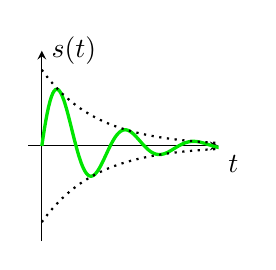
\begin{tikzpicture}
        \begin{axis}
        [   xmin=-0.5,xmax=6.5,
            ymin=-1.5,ymax=1.5
		]
        \addplot[signal,black!10!green] {1.2*sin(2.5*deg(x))*exp(-0.5*x)};
        \addplot[envelop,black]         {1.2*exp(-0.5*x)};
        \addplot[envelop,black]         {-1.2*exp(-0.5*x)};
        \end{axis}
        \end{tikzpicture}
	};
    % pt3
    \node[anchor=south west] at (pt3) {
    	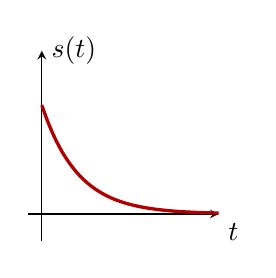
\begin{tikzpicture}
	    \begin{axis}
		[   xmin=-0.5,xmax=6.5,
	        ymin=-0.5,ymax=3
		]
	    \addplot [signal,black!30!red]  {2*exp(-0.75*x)};
	    \end{axis}
	    \end{tikzpicture}
	};
    % pt4
    \node[anchor=south west] at (pt4) {
    	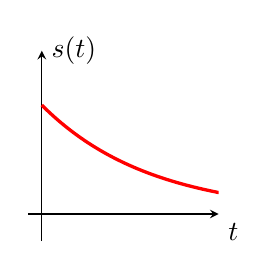
\begin{tikzpicture}
        \begin{axis}
		[	xmin=-0.5,xmax=6.5,
			ymin=-0.5,ymax=3
        ]
        \addplot [signal,red]           {2*exp(-0.25*x)};
        \end{axis}
        \end{tikzpicture}
	};
    % pt5
    \node[anchor=south west] at (pt5) {
    	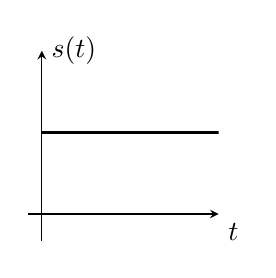
\begin{tikzpicture}
        \begin{axis}
		[	xmin=-0.5,xmax=6.5,
			ymin=-0.5,ymax=3
        ]
        \addplot[signal,black] {1.5};
        \end{axis}
        \end{tikzpicture}
	};
	% pt52
    \node[anchor=south west] at (pt52) {
    	\begin{tikzpicture}
        \begin{axis}
		[	xmin=-0.5,xmax=15,
            ymin=-0.5,ymax=6,
        ]
		\addplot[signal,black] {1+exp(0.1*x)};
        \end{axis}
        \end{tikzpicture}
	};
    % pt6
    \node[anchor=south west] at (pt6) {
    	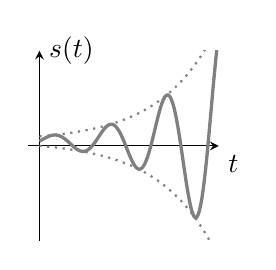
\begin{tikzpicture}
	    \begin{axis}
		[	xmin=-0.5,xmax=8,
            ymin=-20,ymax=20,
        ]
        \addplot[signal,black!50!white]       {sin(2.5*deg(x))*exp(0.40*x)+1};
        \addplot[envelop,black!50!white]      {exp(0.4*x)+1};
        \addplot[envelop,color=black!50!white]{-exp(0.4*x)+1};
        \end{axis}
        \end{tikzpicture}
	};
	% pt62
    \node[anchor=south west] at (pt62) {
    	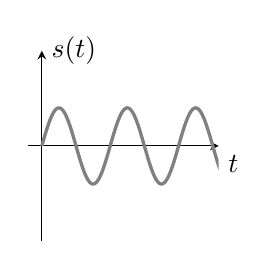
\begin{tikzpicture}
        \begin{axis}
		[	xmin=-0.5,xmax=6.5,
			ymin=-2.5,ymax=2.5,
        ]
        \addplot[signal,black!50!white]       {sin(2.5*deg(x))};
        \end{axis}
        \end{tikzpicture}
	};
    % pt7
    \node[anchor=south west] at (pt7) {
    	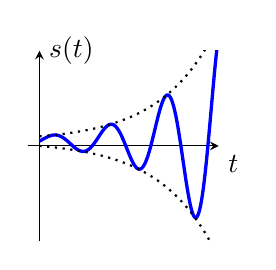
\begin{tikzpicture}
	    \begin{axis}
        [	xmin=-0.5,xmax=8.0,
			ymin=-20,ymax=20
        ]
		\addplot[signal,blue]   {sin(2.5*deg(x))*exp(0.40*x)+1};
		\addplot[envelop,black] {exp(0.4*x)+1};
		\addplot[envelop,black] {-exp(0.4*x)+1};
        \end{axis}
        \end{tikzpicture}
	};
    % pt8
	\node[anchor=south west] at (pt8) {
    	\begin{tikzpicture}
        	\begin{axis}
			[	xmin=-0.5,xmax=15,
				ymin=-0.5,ymax=6,
			]
            \addplot[signal,orange] {1+exp(0.1*x)};
            \end{axis}
            \end{tikzpicture}
	};
        \end{tikzpicture}
    \caption{Stabilité d'un SLCI d'après la carte des pôles de sa fonction de
             transfert et de leurs réponses impulsionnelles. 
             (Vert) Deux pôles complexes conjugués. 
             (Rouge) Pôle à partie réel négative. 
             (Gris) Deux pôles complexes conjugués à partie réelle nulle.
             (Noir) Pôle nul.
             (Bleu) Deux pôles complexes conjugués à partie réelle positive.
             (Orange) Pôle à partie réel positive.}
    \end{figure}
\end{landscape}
\clearpage
\pagestyle{fancy}
\captionsetup{width=0.8\linewidth}
